\section{Visualization with Matplotlib}

Matplotlib is one of the most poplar Python modules used for generating both
static and animated data visualizations. In this section we will focus on
generating static 2D plots with dummy data in order to familiarize ourselves
with the API and how to manipulate different elements of a plot.

To start things off, we will import the relevant modules, namely \texttt{numpy}
and \texttt{matplotlib}. Then, we will use the \texttt{np.linspace()} function
to generate a set of 200 equidistant points between 0 and 100. These will
represent our points on the Ox axis. Based on these samples, we will calculate
the corresponding values of the \texttt{sin()} function and offset them by a
constant.

\begin{lstlisting}[style=pythonstyle]
In [1]: import numpy as np

In [2]: matplotlib.pyplot as plt

In [3]: x = np.linspace(0, 100, 200)

In [4]: x[0], x[-1]
Out[4]: (np.float64(0.0), np.float64(100.0))

In [5]: y1 = np.sin(x) + np.ones(x.size) * 3
\end{lstlisting}

Having generated these values, we can now plot them using Matplotlib. To start
things off, we will create a simple figure that lacks important details such as
labels, a legend or even a title.

\begin{lstlisting}[style=pythonstyle]
In [6]: plt.plot(x, y1)
Out[6]: [<matplotlib.lines.Line2D at 0x7f1dc05d5950>]

In [7]: plt.show()
\end{lstlisting}

\begin{wrapfigure}{l}{0.66 \textwidth}
    \centering
    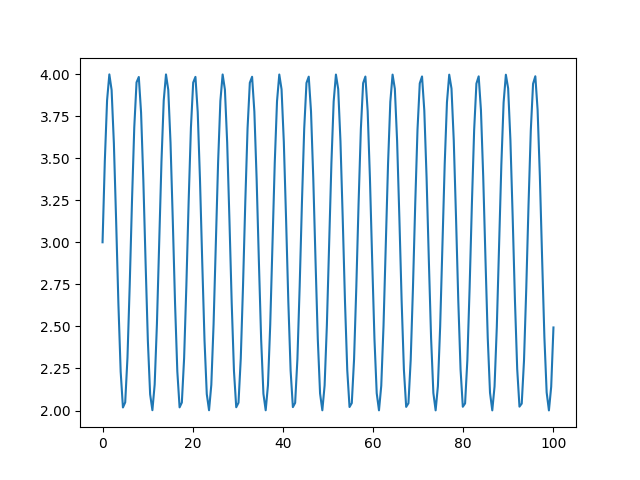
\includegraphics[width=0.55 \textwidth,keepaspectratio]{figures/figure-1.png}
    \caption{A simple plot using the default Matplotlib configurations}
    \label{fig:simple}
\end{wrapfigure}

Although we can discern this as being a sinusoid function, notice the lack of
contextual information. For example, we cannot tell at a glance if the Ox axis
should express and angle or time (as would be the case in signal processing,
for example). Also, the tick intervals are automatically calculated. However,
we might want to set these ourselves. For example, we may wish to tell
Matplotlib to draw the Ox major ticks at intervals of 10 instead of 20. Let us
make a few changes to our previous commands:


\begin{lstlisting}[style=pythonstyle]
In [8]: plt.plot(x, y, 'b-', label='interpolated')
Out[8]: [<matplotlib.lines.Line2D at 0x7f1da7bc8cd0>]

In [9]: plt.plot(x, y, 'ro', label='samples')
Out[9]: [<matplotlib.lines.Line2D at 0x7f1db01f60d0>]

In [10]: plt.xlim(20, 60)
Out[10]: (20.0, 60.0)

In [11]: plt.ylim(2, 4.5)
Out[11]: (2.0, 4.5)

In [12]: plt.xlabel('angle [rad]')
Out[12]: Text(0.5, 0, 'angle [rad]')

In [13]: plt.ylabel('offset sine')
Out[13]: Text(0, 0.5, 'offset sine')

In [14]: plt.title('Example plot')
Out[14]: Text(0.5, 1.0, 'Example plot')

In [15]: plt.legend(loc='upper left')
Out[15]: <matplotlib.legend.Legend at 0x7f1d9c294980>

In [16]: plt.grid(True)

In [17]: plt.show()
\end{lstlisting}

\begin{wrapfigure}{r}{0.66 \textwidth}
    \centering
    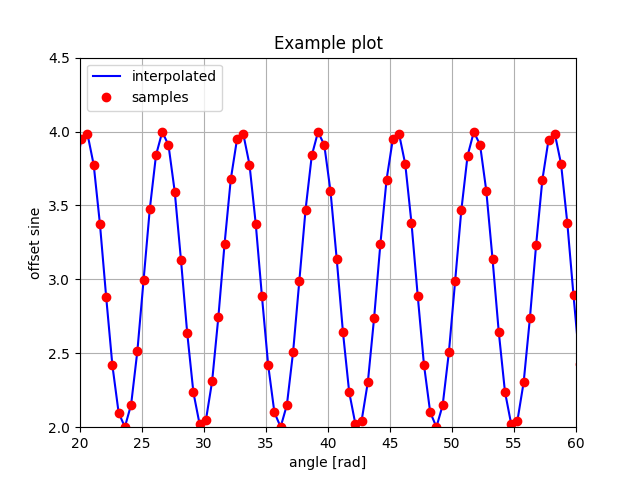
\includegraphics[width=0.55 \textwidth,keepaspectratio]{figures/figure-2.png}
    \caption{More detailed figure containing two plots.}
    \label{fig:simple}
\end{wrapfigure}

In this new version of the plot, we adjusted the Ox and Oy boundaries of the
displayed section. We created more space at the top of the figure to allow us
to draw a legend for the two plots. The first plot consists of a continuous
blue line (\texttt{b-}) that interpolates consecutive discrete samples. The
second plot consists of red dots (\texttt{ro}) representing the exact samples
that we've generated. Make sure to consult the
\href{https://matplotlib.org/stable/api/_as_gen/matplotlib.pyplot.plot.html}
{official documentation} of the \texttt{plt.plot()} function to discover more
tunable parameters. For a more comprehensive tutorial on Matplotlib, check out
\href{https://www.machinelearningplus.com/plots/matplotlib-tutorial-complete-guide-python-plot-examples/}
{this resource}.

